\documentclass{article}
\PassOptionsToPackage{numbers,compress}{natbib}
\usepackage[final]{neurips}
\usepackage[utf8]{inputenc}
\usepackage[T1]{fontenc}
\usepackage{booktabs}
\usepackage{amsmath,amsfonts,amssymb}
\usepackage{graphicx}
\usepackage{microtype}
\usepackage{xcolor}
\usepackage{array}
\usepackage{float}
\usepackage{enumitem}
\usepackage[hidelinks]{hyperref}
\setlist{nosep,leftmargin=*}
\setlength{\textfloatsep}{4pt plus 1pt minus 1pt}
\setlength{\floatsep}{3pt plus 1pt minus 1pt}
\setlength{\intextsep}{3pt plus 1pt minus 1pt}
\newcommand{\R}{\mathbb{R}}

\title{Learning Spatial Unit-Norm Latents with Riemannian Flow Matching}
\author{Mohammadreza Tavasoli Naeini \\
Department of Electrical and Computer Engineering, University of Toronto \\
\texttt{mohammadreza.tavasolinaeini@mail.utoronto.ca}}

\begin{document}
\maketitle

\begin{abstract}
Latent generative models often use a Gaussian prior, but an autoencoder can learn a different latent geometry. We study a simple rule: the prior should match the latent space learned by the autoencoder. Spherical Riemannian Unit-Norm Latents (SRUL) learns a spatial grid of unit-norm tokens. During autoencoder training, random tangent perturbations make the decoder robust and encourage the token directions to cover each sphere approximately uniformly; the perturbation scale $\sigma_{\mathrm{enc}}$ also acts as an information-control knob. Riemannian Flow Matching (RFM) then learns the remaining structured distribution using geodesic paths on the same spherical support. We evaluate geometry matching, information control, classifier-free guidance, and transfer to CIFAR-10, PathMNIST, and CelebA-64.
\end{abstract}

\section*{Attestation of Teamwork}
Mohammadreza Tavasoli Naeini conducted the background study, designed and implemented the models, ran and analyzed the experiments, and prepared the report, presentation, and code.

\section{Introduction}
Latent generative models have two parts. An autoencoder first maps an image to a latent code, and a prior then learns how to generate new codes for the decoder. Gaussian latents are common, especially in VAE-based models, but the encoder is free to learn a different geometry. Normalization can make token norms nearly constant, so information is carried mainly by direction. Transformer encoders with LayerNorm are one example, and explicit $L_2$ normalization can create the same structure in a convolutional encoder.

The prior should therefore be chosen after considering the latent support. When an encoder produces spherical tokens, standard linear interpolation is not well matched to them: even if both endpoints have unit norm, the straight path is a chord through the sphere's interior. The reverse mismatch can also occur. A VAE may use both token direction and token magnitude; projecting its latents onto a sphere after training removes the magnitude information that its decoder expects.

To study this support-matching principle, we introduce Spherical Riemannian Unit-Norm Latents (SRUL). Its autoencoder learns a spatial grid of unit-norm tokens. We train the decoder with random tangent perturbations so nearby spherical codes reconstruct consistently, and we also use larger random perturbations to encourage approximately uniform coverage of each token sphere. RFM then learns the remaining spatial structure on the same product of spheres. The representation and prior are therefore designed for the same latent geometry.

We study the design with two controlled tests. First, we keep the spherical autoencoder unchanged and compare a Euclidean chord with geodesic RFM transport. Second, we compare SRUL with a VAE modeled by standard FM and with the same VAE after its latents are reduced to directions for projected RFM. The second test shows whether a spherical prior can be attached to a VAE after training without losing radial information. We use the tangent-noise scale as an information-control knob, study classifier-free guidance, and evaluate the same pipeline on CIFAR-10, PathMNIST, and CelebA-64.

\section{Related Work and Positioning}
Variational autoencoders learn stochastic Euclidean latents and use a KL term to regularize them toward a Gaussian prior \cite{vae}. Latent Diffusion Models move generation from pixels to a learned latent grid, reducing computation while preserving perceptually important information \cite{ldm}. Unified Latents studies information control through encoder noise \cite{ul}. Sphere Encoder studies spherical latent representations and noisy spherical training \cite{sphere}. SRUL combines these ideas in a spatial product-of-spheres representation and learns its prior with RFM.

Flow Matching learns a time-dependent velocity field along a chosen probability path \cite{fm}. Standard linear Flow Matching uses straight paths in Euclidean latent space. RJF observes that normalized representation encoders often produce features with nearly constant norm and replaces this interpolation with Riemannian Flow Matching on the sphere; it also studies an additional Jacobi weighting \cite{rjf}. SRUL differs in two ways. It learns the spatial spherical representation rather than assuming a pretrained representation encoder, and it uses tangent perturbation as a controllable latent bottleneck. This makes encoder--prior co-design, rather than only applying RFM to an existing representation, the central question. The final method uses the RFM formulation because it was the strongest variant in our experiments.

\section{Method}
\subsection{Pipeline overview}
Figure~\ref{fig:pipeline} shows the full pipeline. The encoder produces unit-norm spatial tokens. Tangent perturbations have two roles during autoencoder training: small perturbations control how much image information is retained, while larger random perturbations encourage approximately uniform token coverage and a robust decoder. RFM then learns the remaining latent structure using geodesic paths and tangent velocities. During sampling, spherical noise is transported with exponential-map steps and decoded into a new image.

\begin{figure}[H]
\centering
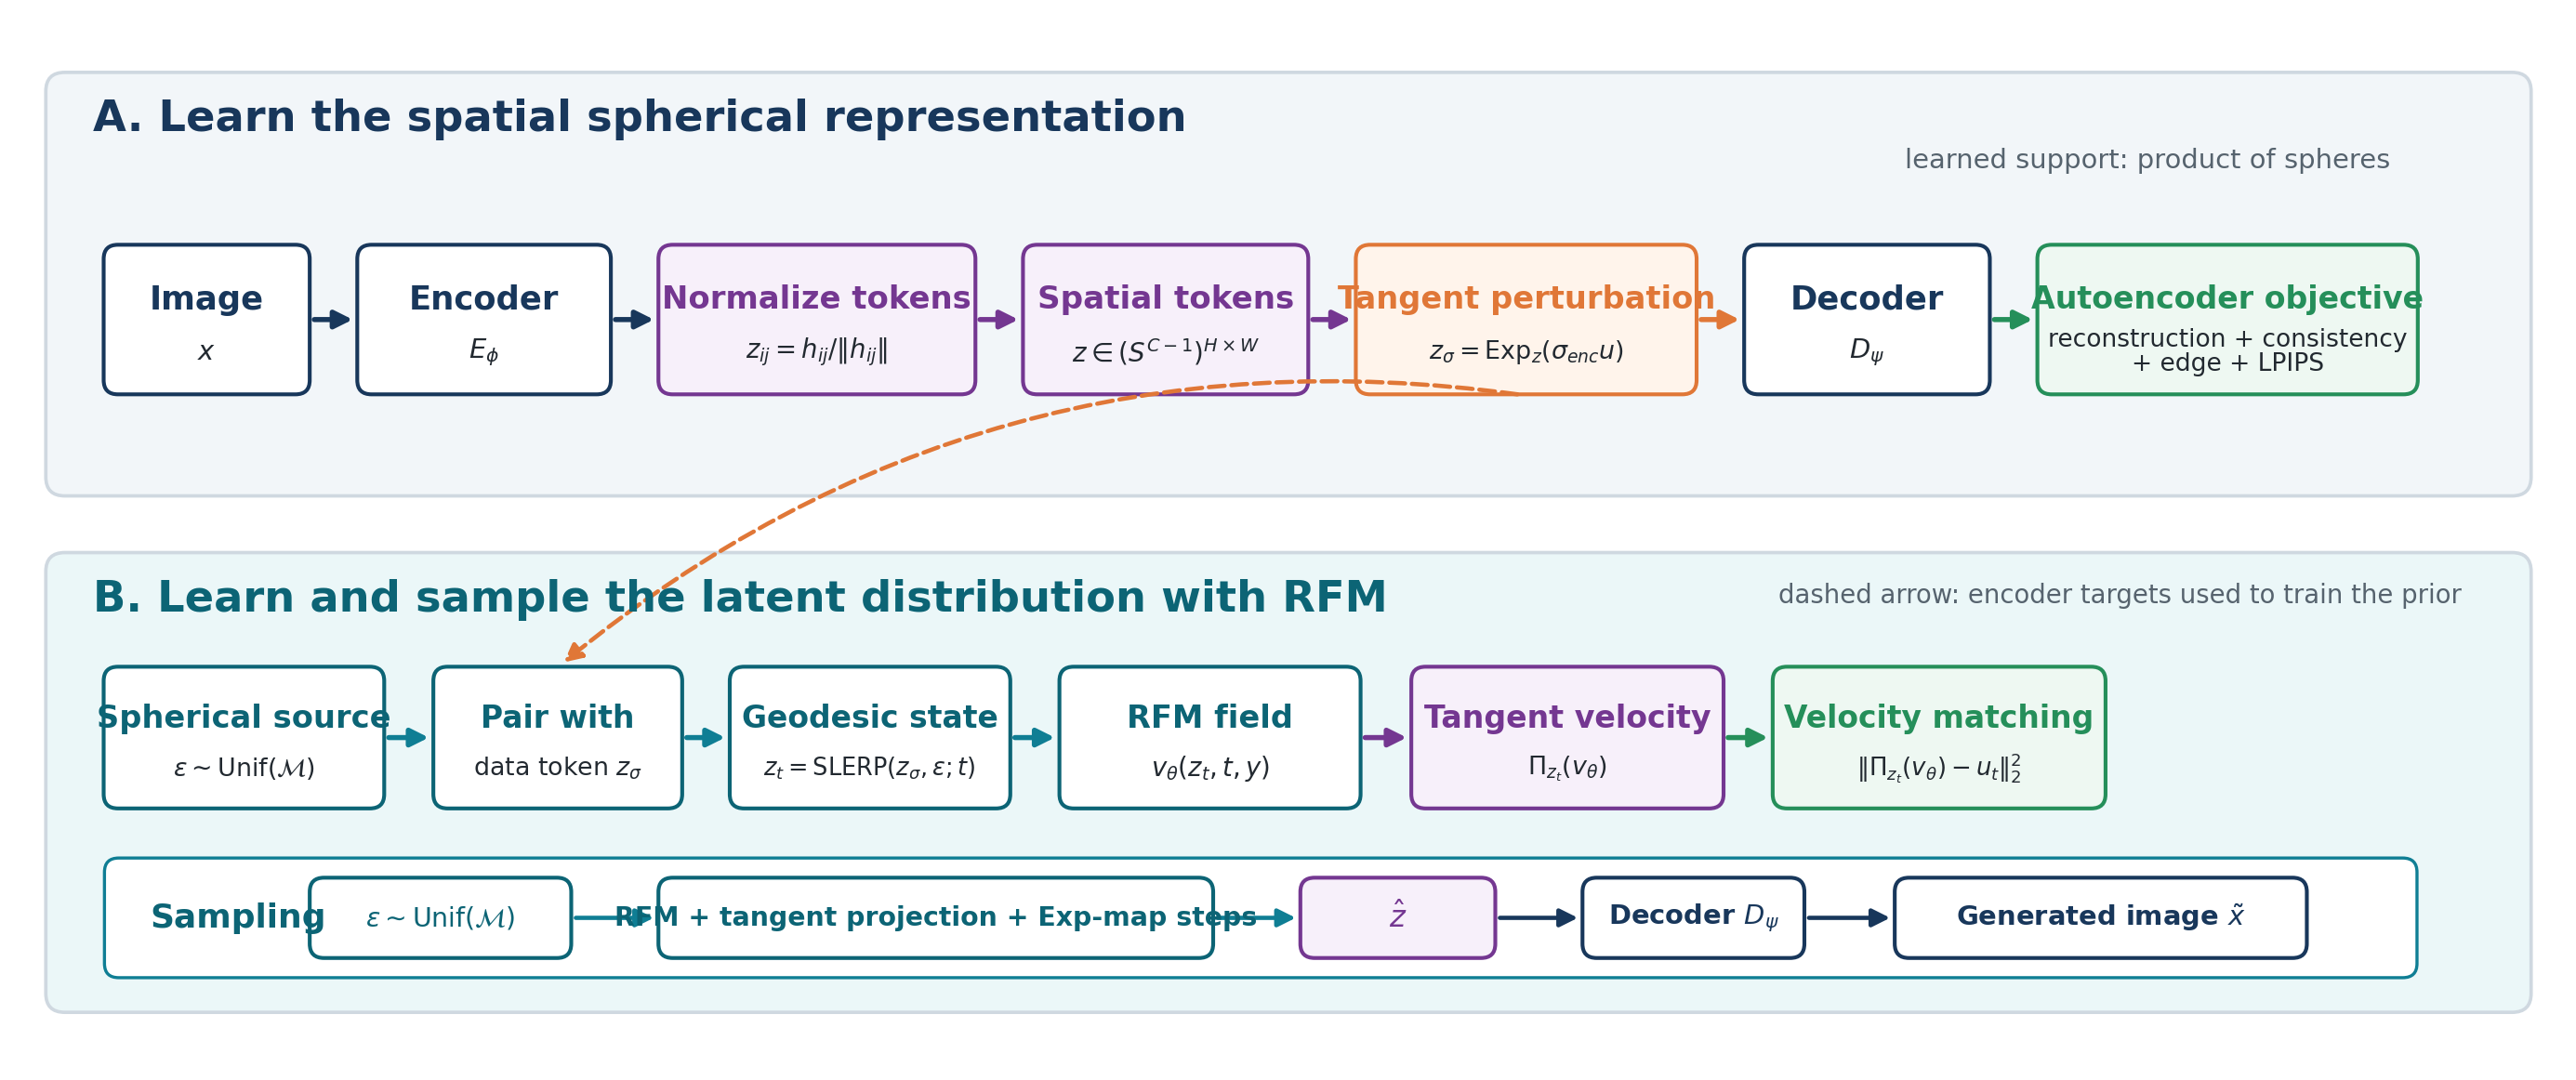
\includegraphics[width=0.95\linewidth]{assets/srul_pipeline_v10.png}
\caption{SRUL pipeline. The autoencoder learns spatial unit-norm tokens with tangent perturbations for information control, approximately uniform token coverage, and decoder robustness. RFM then learns and samples the remaining structured distribution on the same product-of-spheres manifold.}
\label{fig:pipeline}
\end{figure}

\subsection{Spatial spherical autoencoder}
For an image $x$, the encoder produces a spatial tensor
\begin{equation}
 h=E_\phi(x)\in\R^{C\times H\times W},\qquad
 z_{:,i,j}=\frac{h_{:,i,j}}{\|h_{:,i,j}\|_2}\in S^{C-1}.
\label{eq:encoder}
\end{equation}
The full latent space is $\mathcal M=(S^{C-1})^{HW}$. We use $C=32$, a $4\times4$ token grid for $32\times32$ images, and an $8\times8$ grid for CelebA-64. Unit normalization puts every token on a sphere, but by itself it does not stop the encoder from using only a small angular region. We therefore train with random tangent rotations. A smaller rotation must still reconstruct the input image, while a larger rotation is encouraged to decode consistently with the smaller one. This makes the decoder valid over a wider part of the sphere and encourages approximately uniform token coverage, $q_\phi(z_{i,j})\approx\operatorname{Unif}(S^{C-1})$. This is a marginal goal, not an independent uniform distribution for the full grid: spatial dependencies can remain and are learned later by RFM. Appendix~\ref{app:uniform} gives the training details.

For broad coverage, we use the same random tangent direction $u$ to make a small and a larger rotation,
\begin{equation}
 z_{\mathrm{S}}=\operatorname{Exp}_{z}(\alpha_{\mathrm{S}}u),\qquad
 z_{\mathrm{L}}=\operatorname{Exp}_{z}(\alpha_{\mathrm{L}}u),\qquad
 \alpha_{\mathrm{S}}<\alpha_{\mathrm{L}}.
\end{equation}
The small rotation must reconstruct the input, while the larger one should decode to a similar image. We train with a simple combination
\begin{equation}
 \mathcal L_{\mathrm{AE}}
 =\mathcal L_{\mathrm{recon}}+\lambda_{\mathrm{cons}}\mathcal L_{\mathrm{cons}}
 +\lambda_{\mathrm{lat}}\mathcal L_{\mathrm{lat}}
 +\lambda_p\mathcal L_{\mathrm{LPIPS}}+\lambda_e\mathcal L_{\mathrm{edge}}.
\label{eq:ae}
\end{equation}
Here, reconstruction keeps image content, $\mathcal L_{\mathrm{cons}}$ makes the large-rotation output agree with the small-rotation output, LPIPS preserves perceptual shape and texture, the edge term preserves local boundaries, and latent consistency makes the perturbed round trip return near the clean token directions. Together these losses make a wider spherical neighborhood usable by the decoder and encourage token directions to spread more uniformly instead of concentrating in a narrow region. Appendix~\ref{app:ae} gives the loss interpretation and Appendix~\ref{app:uniform} gives the coverage details.

\subsection{Tangent-noise information control}
For each token, Gaussian noise is projected onto the tangent space,
\begin{equation}
 \xi\sim\mathcal N(0,I),\qquad
 u=\Pi_z(\xi)=\xi-\langle\xi,z\rangle z,
\end{equation}
and the perturbed token is
\begin{equation}
 z_\sigma=\operatorname{Exp}_z(\sigma_{\mathrm{enc}}u).
\label{eq:noise}
\end{equation}
For a tangent vector $v$, the spherical exponential map is
\begin{equation}
 \operatorname{Exp}_z(v)=\cos(\|v\|_2)z+\sin(\|v\|_2)\frac{v}{\|v\|_2}.
\label{eq:exp}
\end{equation}
Because $v\perp z$, this is a rotation and its output still has unit norm. The scalar $\sigma_{\mathrm{enc}}$ is an information-control knob: larger values perturb directions more strongly and retain less image-specific information. Appendix~\ref{app:exp} gives the norm proof and sampling interpretation.

\subsection{Riemannian Flow Matching prior}
Standard linear Flow Matching connects a source $\epsilon$ and target $z$ with $x_t=(1-t)\epsilon+tz$, whose target velocity is $z-\epsilon$. RFM keeps this velocity-regression idea but replaces the straight path with a manifold geodesic. Its source is factorized uniform spherical noise, $p_0=\prod_{i,j}\operatorname{Unif}(S^{C-1})$, while its target is the structured joint distribution $q_\phi(z)$ or $q_\phi(z\mid y)$; individual token marginals are encouraged to be approximately uniform, but spatial dependencies can remain. For a data latent $z_\sigma$ and source sample $\epsilon\sim p_0$, the tokenwise geodesic is
\begin{equation}
 z_t=\operatorname{SLERP}(z_\sigma,\epsilon;t)
 =\frac{\sin((1-t)\Omega)}{\sin\Omega}z_\sigma
 +\frac{\sin(t\Omega)}{\sin\Omega}\epsilon,
\quad \Omega=\arccos(z_\sigma^\top\epsilon).
\label{eq:slerp}
\end{equation}
SLERP is a constant-speed rotation in the two-dimensional plane of its endpoints. Therefore $\|z_t\|_2=1$ for every $t$, and the curve is the great-circle geodesic; Appendix~\ref{app:fm} gives a direct proof. Let $u_t=\partial z_t/\partial t$ be the known target tangent velocity. We train
\begin{equation}
 \mathcal L_{\mathrm{RFM}}
 =\mathbb E\!\left[\left\|\Pi_{z_t}\big(v_\theta(z_t,t)\big)-u_t\right\|_2^2\right].
\label{eq:rfm}
\end{equation}
Thus RFM training is supervised velocity regression: a random point on a known geodesic is constructed, its exact velocity is computed, and the network is trained to predict that velocity after tangent projection. During sampling, the target endpoint is no longer known; the model starts from spherical noise and repeatedly follows its learned field,
\begin{equation}
 z_{t-\Delta t}=\operatorname{Exp}_{z_t}\!\left(-\Delta t\,\Pi_{z_t}(v_\theta)\right),
\label{eq:sample}
\end{equation}
so every intermediate token remains on its sphere.

\subsection{Conditional generation and classifier-free guidance}
The field may also receive a label $y$, giving $v_\theta(z_t,t,y)$. During training, the label is replaced by a null label with probability $0.1$. During sampling,
\begin{equation}
 v_{\mathrm{CFG}}=v_\theta(z_t,t,\varnothing)
+s\big[v_\theta(z_t,t,y)-v_\theta(z_t,t,\varnothing)\big].
\label{eq:cfg}
\end{equation}
Bayes rule motivates separating an unconditional component from a label-specific component in classifier guidance. CFG learns both components in one network by randomly dropping labels, then amplifies their difference during sampling \cite{cfg}. The guided field is projected before every exponential-map update, so conditioning changes sampling strength but not the manifold. Larger $s$ usually pushes samples toward more class-typical regions, which can improve FID and precision while reducing coverage and recall; Appendix~\ref{app:cfg} explains this relation carefully.

\section{Experiments}
\subsection*{Setup}
CIFAR-10 is used for controlled geometry and support-matching tests \cite{cifar}. PathMNIST evaluates transfer to histopathology texture \cite{medmnist}, and CelebA-64 evaluates a larger $64\times64$ setting \cite{celeba}. We use AdamW in both training stages and 100 integration steps for final sampling. We report FID, KID, feature precision and recall, and token norm. The stronger approximately-uniform coverage training was added after the current quantitative runs, so the numerical tables below remain the measured base SRUL results until that rerun is completed.

\subsection*{Does the encoder--prior geometry match?}
We test the same design principle at two levels. The first experiment asks whether transport remains on a spherical support that is already defined by the encoder. The second asks whether a spherical direction-only prior can be attached after a Euclidean autoencoder has learned a different support.

\paragraph{Transport on spherical support.}
The path comparison uses the same spherical encoder, decoder, source distribution, latent size, prior capacity, and training budget. Only the path changes. The baseline uses
\begin{equation}
 z_t^{\mathrm{chord}}=(1-t)z_\sigma+t\epsilon.
\end{equation}
Although both endpoints have unit norm, the chord enters the sphere. For nearly orthogonal endpoints, its midpoint norm is approximately $1/\sqrt2=0.707$; the measured minimum mean norm is $0.705$. SRUL follows SLERP and remains at norm $1$.

\begin{figure}[H]
\centering
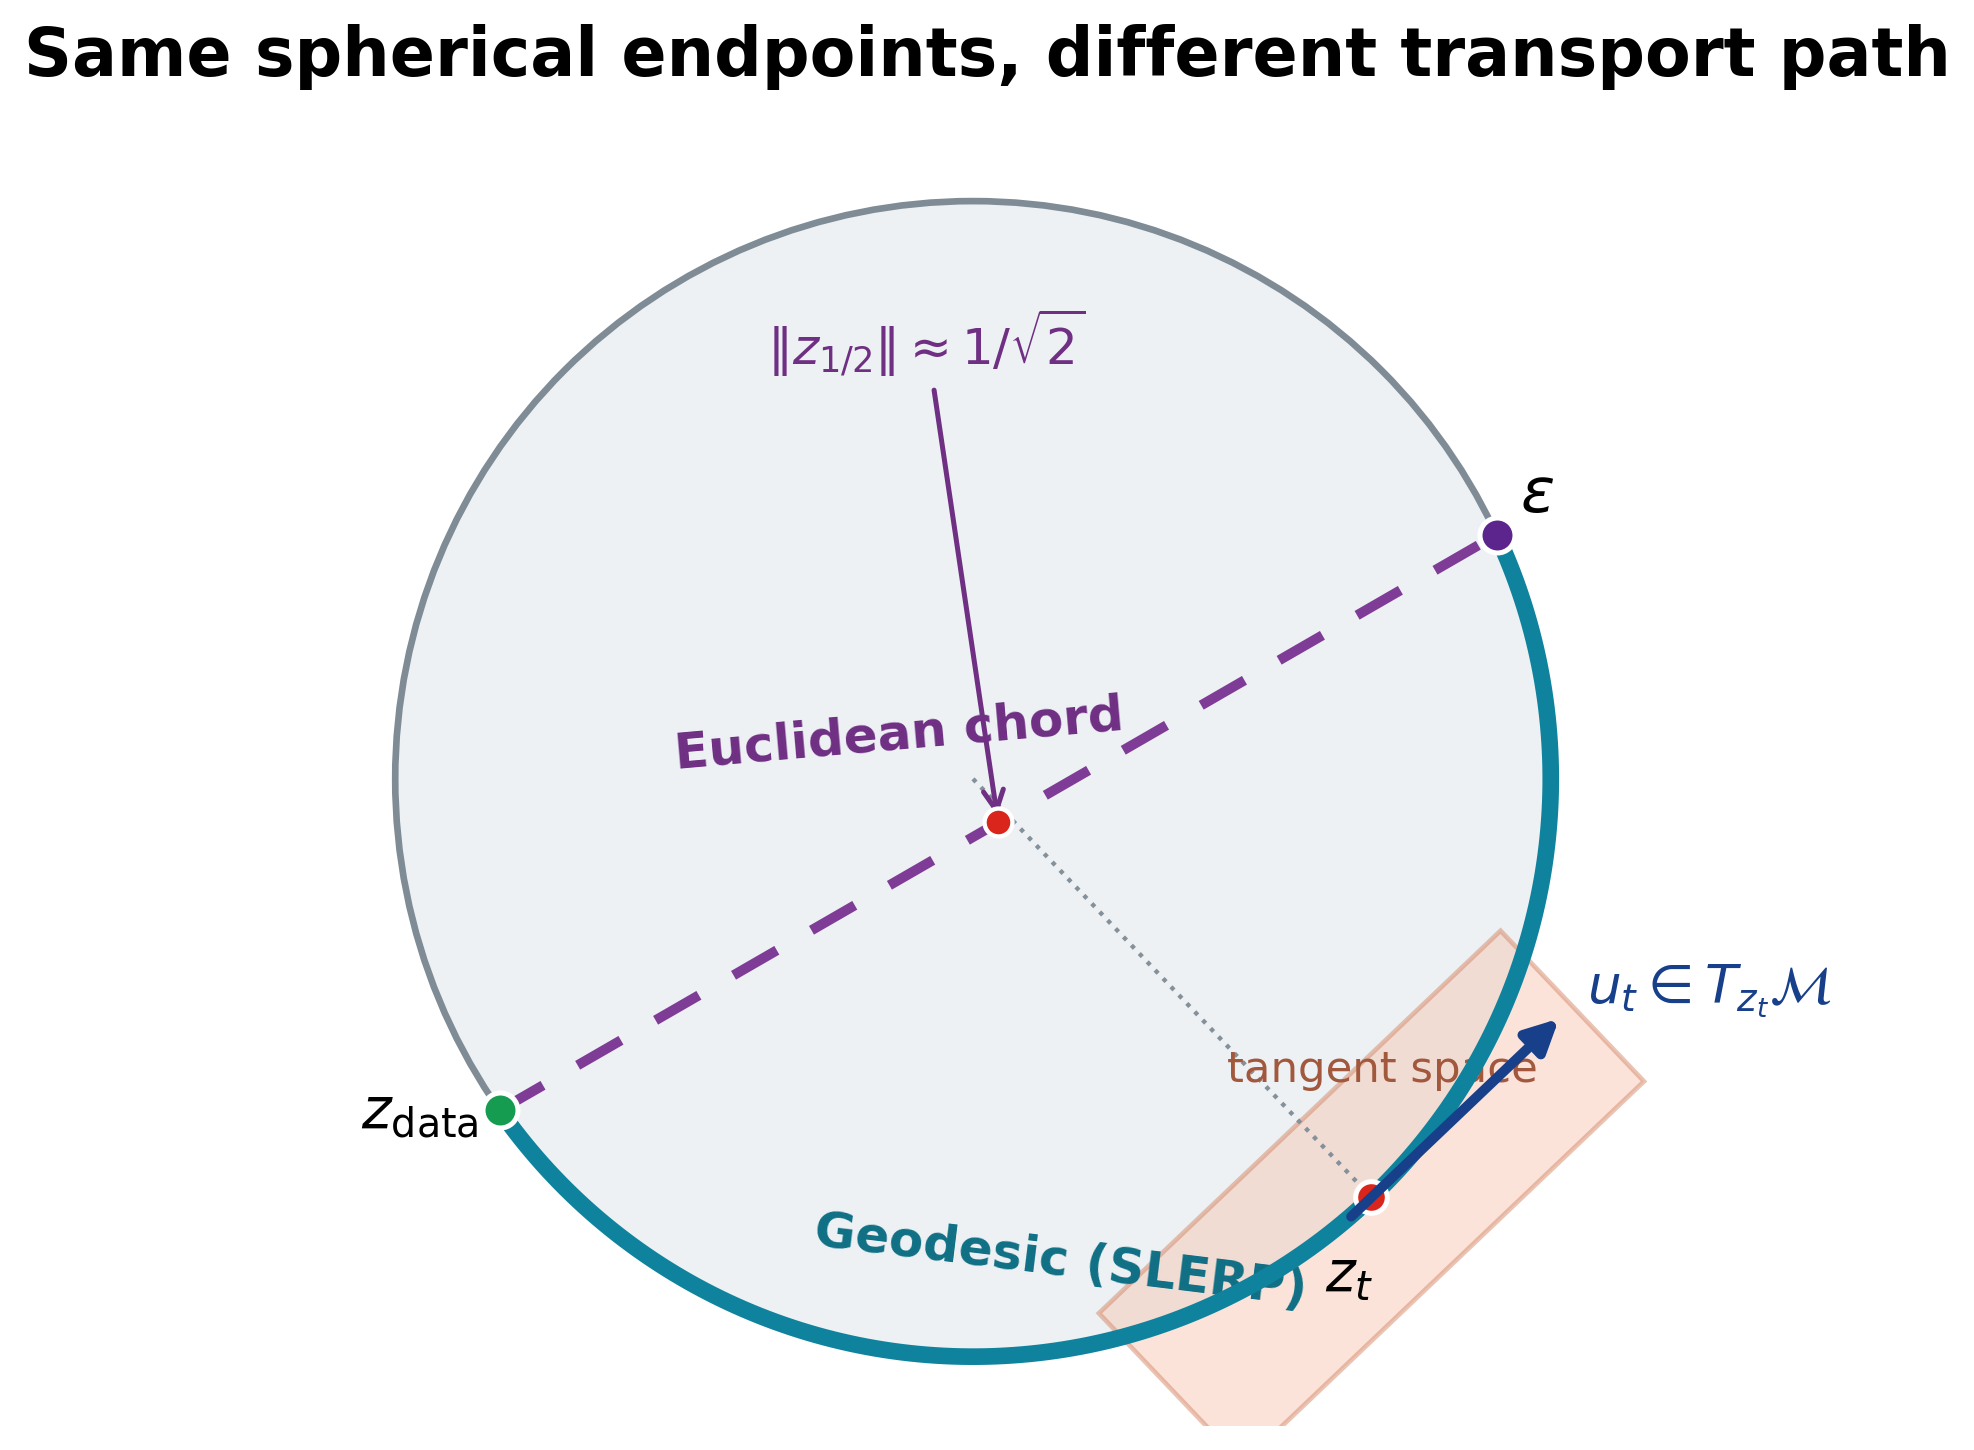
\includegraphics[width=0.55\linewidth]{assets/geometry_schematic_v9_clean.png}
\caption{With the same spherical encoder, the chord visits interior states while SRUL follows the geodesic and keeps its velocity in the tangent space.}
\label{fig:geometry}
\end{figure}

\begin{table}[H]
\centering
\small
\caption{CIFAR-10 path comparison with the same spherical autoencoder.}
\label{tab:geometry}
\setlength{\tabcolsep}{8pt}
\begin{tabular}{lrrrrr}
\toprule
Method & FID$\downarrow$ & KID$\downarrow$ & Precision$\uparrow$ & Recall$\uparrow$ & Min. norm$\uparrow$ \\
\midrule
Chord baseline & 67.44 & 0.0740 & 0.840 & 0.085 & 0.705 \\
\textbf{SRUL} & \textbf{63.84} & \textbf{0.0667} & \textbf{0.857} & \textbf{0.091} & \textbf{1.000} \\
\bottomrule
\end{tabular}
\end{table}
The geodesic improves all four image metrics and removes the radial excursion. This isolates the benefit of matching the transport path to an already-spherical representation.

\paragraph{Support matching with the same VAE.}
A VAE latent is Euclidean and can use both token direction and magnitude. With the same trained VAE, standard FM models the full token $z$, while projected RFM keeps only $u=z/\|z\|_2$ and restores a class/token mean radius. SRUL is included because it learns spherical support before RFM.

\begin{table}[H]
\centering
\small
\caption{CIFAR-10 support-matching comparison (CFG $s=2$).}
\label{tab:support}
\setlength{\tabcolsep}{6pt}
\begin{tabular}{p{2.75cm}p{4.2cm}rrr}
\toprule
Method & Latent support and prior & FID$\downarrow$ & Precision$\uparrow$ & Recall$\uparrow$ \\
\midrule
\textbf{SRUL} & Spherical autoencoder + RFM & \textbf{49.42} & \textbf{0.857} & \textbf{0.110} \\
VAE + standard FM & Full VAE latent + linear FM & 50.70 & 0.855 & 0.091 \\
VAE + projected RFM & Directions + class/token mean radius & 56.04 & 0.848 & 0.063 \\
\bottomrule
\end{tabular}
\end{table}

Projected RFM is worse because post-hoc normalization removes radial information used by the VAE decoder; Appendix~\ref{app:ae} gives the supporting latent-consistency interpretation.

\subsection*{Information-control and guidance ablations}
We use two controlled studies: the information-control sweep fixes CFG at $s=2$, while the guidance sweep fixes $\sigma_{\mathrm{enc}}=0.15$.

\begin{table}[H]
\centering
\scriptsize
\caption{CIFAR-10 controlled ablations. The left block fixes CFG at $s=2$; the right block fixes $\sigma_{\mathrm{enc}}=0.15$.}
\label{tab:controls}
\setlength{\tabcolsep}{4.1pt}
\begin{tabular}{crrr|crrr}
\toprule
$\sigma_{\mathrm{enc}}$ & Recon. FID$\downarrow$ & Gen. FID$\downarrow$ & Recall$\uparrow$ & CFG $s$ & FID$\downarrow$ & Precision$\uparrow$ & Recall$\uparrow$ \\
\midrule
0.05 & \textbf{17.53} & \textbf{48.71} & 0.090 & 1.0 & 62.44 & 0.854 & \textbf{0.083} \\
0.15 & 19.56 & 51.61 & \textbf{0.090} & 1.5 & 54.83 & 0.865 & 0.071 \\
0.30 & 27.85 & 58.16 & 0.073 & 2.0 & \textbf{49.39} & \textbf{0.884} & 0.059 \\
\bottomrule
\end{tabular}
\end{table}
Appendix~\ref{app:crosssweep} applies the same controlled slices to PathMNIST and CelebA-64. Large noise ($0.30$) harms all datasets; guidance helps CIFAR-10 strongly, peaks at $s=1.5$ on PathMNIST, and changes CelebA-64 only slightly.

\subsection*{Evaluation across image domains}
\begin{table}[H]
\centering
\scriptsize
\caption{SRUL evaluation under the same reference setting, $\sigma_{\mathrm{enc}}=0.15$ and CFG $s=2$.}
\label{tab:domains}
\setlength{\tabcolsep}{2.8pt}
\renewcommand{\arraystretch}{1.08}
\begin{tabular}{p{1.25cm}p{3.0cm}p{1.1cm}rrrr}
\toprule
Dataset & Role in the study & Grid & Recon. FID & Gen. FID & Precision & Recall \\
\midrule
CIFAR-10 & Natural-object geometry and sampling study & $4\times4$ & 17.31 & 49.39 & 0.884 & 0.059 \\
PathMNIST & Histopathology texture transfer & $4\times4$ & 7.13 & 29.36 & 0.829 & 0.309 \\
CelebA-64 & $64\times64$ facial-image scale-up & $8\times8$ & 9.08 & 41.22 & 0.657 & 0.198 \\
\bottomrule
\end{tabular}
\end{table}
The same reference operating point transfers across natural objects, histopathology textures, and a larger facial-image setting.

\section{Conclusion}
SRUL co-designs a unit-norm spatial autoencoder and an RFM prior on the same support. Geodesic transport improves over a chord, projected RFM underperforms when applied after VAE training, and controlled sweeps show that excessive tangent noise hurts all datasets while guidance is dataset dependent.

\clearpage
{\small
\begin{thebibliography}{12}
\bibitem{vae} D. P. Kingma and M. Welling. Auto-Encoding Variational Bayes. ICLR, 2014.
\bibitem{ldm} R. Rombach, A. Blattmann, D. Lorenz, P. Esser, and B. Ommer. High-resolution image synthesis with latent diffusion models. CVPR, 2022.
\bibitem{fm} Y. Lipman, R. T. Q. Chen, H. Ben-Hamu, M. Nickel, and M. Le. Flow matching for generative modeling. ICLR, 2023.
\bibitem{rjf} A. Kumar and V. M. Patel. Learning on the Manifold: Unlocking Standard Diffusion Transformers with Representation Encoders. arXiv, 2026.
\bibitem{sphere} Z. Yue et al. Image Generation with a Sphere Encoder. arXiv, 2026.
\bibitem{ul} J. Heek et al. Unified Latents: Controlling Information Flow in Latent Generative Models. arXiv, 2026.
\bibitem{cifar} A. Krizhevsky. Learning Multiple Layers of Features from Tiny Images. Technical report, 2009.
\bibitem{medmnist} J. Yang, R. Shi, D. Wei, et al. MedMNIST v2: A Large-Scale Lightweight Benchmark for 2D and 3D Biomedical Image Classification. Scientific Data, 2023.
\bibitem{celeba} Z. Liu, P. Luo, X. Wang, and X. Tang. Deep Learning Face Attributes in the Wild. ICCV, 2015.
\bibitem{lpips} R. Zhang, P. Isola, A. A. Efros, E. Shechtman, and O. Wang. The Unreasonable Effectiveness of Deep Features as a Perceptual Metric. CVPR, 2018.
\bibitem{cfg} J. Ho and T. Salimans. Classifier-Free Diffusion Guidance. arXiv:2207.12598, 2022.
\end{thebibliography}}


\clearpage
\appendix
\section{Autoencoder losses in detail}
\label{app:ae}
The autoencoder loss in Eq.~\eqref{eq:ae} combines image-level fidelity with latent-space stability. The terms have different roles and should not be interpreted as interchangeable versions of the same error.

\paragraph{Pixel, edge, and perceptual losses.}
The clean and noisy $L_1$ terms compare corresponding pixels. They preserve color, brightness, and approximate spatial location, but pixel distance can penalize a small shift strongly and can also reward blurry averages. The edge loss compares horizontal and vertical image gradients, so it gives direct pressure to preserve boundaries and local structure. LPIPS instead passes the real and reconstructed images through a frozen pretrained feature network and compares normalized features at several layers \cite{lpips}. A simplified form is
\begin{equation}
 \mathcal L_{\mathrm{LPIPS}}(x,\hat x)
 =\sum_{\ell}\frac{1}{H_\ell W_\ell}
 \sum_p\left\|w_\ell\odot
 \big(\bar f_\ell(x)_p-\bar f_\ell(\hat x)_p\big)\right\|_2^2.
\end{equation}
Early features respond to edges and textures, while deeper features respond to larger visual patterns. The feature network is frozen; gradients pass through it only to update the SRUL encoder and decoder.

\paragraph{Latent consistency.}
Let
\begin{equation}
 \tilde z=E_\phi\big(D_\psi(z_\sigma)\big).
\end{equation}
The latent-consistency term is the average cosine distance between the clean token $z$ and the re-encoded noisy reconstruction $\tilde z$:
\begin{equation}
 \mathcal L_{\mathrm{lat}}
 =1-\frac{1}{BHW}\sum_{b,i,j}z_{b,i,j}^{\top}\tilde z_{b,i,j}.
\end{equation}
Because both tokens are unit norm, their dot product is exactly the cosine of their angle. A loss of zero means that the noisy round trip returns to the same token direction. In the implementation, the clean $z$ is treated as a stopped-gradient target for this branch. The term therefore acts as a local denoising and cycle-consistency constraint: nearby spherical codes should decode to the same image content and re-encode near the same clean representation.


\section{Broad spherical coverage during autoencoder training}
\label{app:uniform}
To encourage broad spherical coverage, SRUL creates two perturbed versions of the same latent grid along one random tangent direction $u$. One perturbation is small and one is larger. The small perturbation must reconstruct the image, while the large perturbation must decode consistently with the small one. We normalize the full tangent grid so that $\|u\|_{\mathcal M}=1$ and write the two codes as
\begin{equation}
 z_{\mathrm{L}}=\operatorname{Exp}_{z}(\alpha u),\qquad
 z_{\mathrm{S}}=\operatorname{Exp}_{z}(s\alpha u).
\end{equation}

Let $\hat x_{\mathrm{S}}=D_\psi(z_{\mathrm{S}})$ and $\hat x_{\mathrm{L}}=D_\psi(z_{\mathrm{L}})$. The adapted loss is
\begin{align}
 \mathcal L_{\mathrm{spread}}={}&
 \mathcal L_{\mathrm{rec}}(\hat x_{\mathrm{S}},x)
 +\lambda_{\mathrm{pix}}\mathcal L_{\mathrm{rec}}
 \big(\hat x_{\mathrm{L}},\operatorname{sg}(\hat x_{\mathrm{S}})\big)\\
 &+\lambda_{\mathrm{lat}}
 \left[1-\cos\!\left(z,E_\phi(\hat x_{\mathrm{L}})\right)\right],
\end{align}
where $\mathcal L_{\mathrm{rec}}$ combines Smooth-$L_1$ and LPIPS, and $\operatorname{sg}$ denotes stop-gradient. The small-noise branch anchors image reconstruction, the large-noise branch enlarges the decodable neighborhood, and the latent term maps distorted outputs back toward the clean code. Across many images, the wider neighborhoods discourage token directions from clustering in one angular region and encourage approximately uniform coverage of each token sphere.

\section{From standard Flow Matching to spherical RFM}
\label{app:fm}
\subsection{Standard linear Flow Matching}
Let $\epsilon\sim p_0$ be a simple source and $z\sim p_1$ a target latent. Standard linear Flow Matching chooses
\begin{equation}
 x_t=(1-t)\epsilon+tz,\qquad
 u_t=\frac{\partial x_t}{\partial t}=z-\epsilon.
\end{equation}
A neural field is trained by
\begin{equation}
 \mathcal L_{\mathrm{FM}}
 =\mathbb E\big[\|v_\theta(x_t,t)-u_t\|_2^2\big].
\end{equation}
At inference, one samples $x_0\sim p_0$ and solves the ODE $\dot x_t=v_\theta(x_t,t)$. Training is called simulation-free because a full ODE trajectory is not solved for every update: one samples $t$, constructs $x_t$ directly, and regresses its known velocity \cite{fm}.

\subsection{Why SLERP is the spherical geodesic}
Let $a,b\in S^{d-1}$, let $\Omega=\arccos(a^\top b)$, and assume $0<\Omega<\pi$. Define
\begin{equation}
 q=\frac{b-\cos\Omega\,a}{\sin\Omega}.
\end{equation}
Then $q\perp a$, $\|q\|_2=1$, and $b=\cos\Omega\,a+\sin\Omega\,q$. Substituting this expression into Eq.~\eqref{eq:slerp} gives
\begin{equation}
 \gamma(t)=\cos(t\Omega)a+\sin(t\Omega)q.
\end{equation}
This is a rotation through angle $t\Omega$ in the plane spanned by the endpoints. Since $a$ and $q$ are orthonormal,
\begin{equation}
 \|\gamma(t)\|_2^2=\cos^2(t\Omega)+\sin^2(t\Omega)=1.
\end{equation}
The speed is constant, $\|\dot\gamma(t)\|_2=\Omega$, and
\begin{equation}
 \ddot\gamma(t)=-\Omega^2\gamma(t).
\end{equation}
On the unit sphere, $\gamma(t)$ is the normal direction. Hence the acceleration has no tangential component, which is the geodesic equation. For non-antipodal endpoints, this great-circle arc is the unique shortest geodesic.

\subsection{RFM target and loss}
Differentiating SLERP gives the tokenwise target velocity
\begin{equation}
 u_t=\frac{\Omega}{\sin\Omega}
 \left[-\cos((1-t)\Omega)a+\cos(t\Omega)b\right].
\end{equation}
Because $\|\gamma(t)\|_2=1$, differentiating the norm gives $\gamma(t)^\top u_t=0$; the target is tangent. The neural network may output a radial component, so its prediction is projected as
\begin{equation}
 \Pi_z(v)=v-(z^\top v)z.
\end{equation}
Equation~\eqref{eq:rfm} then matches the projected prediction to the exact tangent velocity and averages the error over the batch and all spatial tokens.

\section{Exponential-map sampling}
\label{app:exp}
At inference there is no paired target latent. Sampling starts from $z_0\sim\operatorname{Unif}(\mathcal M)$ and repeatedly queries the learned field. A direct Euler step is not manifold preserving. Even when $v\perp z$ and $\|z\|_2=1$,
\begin{equation}
 \|z+\Delta t\,v\|_2^2=1+\Delta t^2\|v\|_2^2>1.
\end{equation}
The exponential map instead performs a geodesic step:
\begin{equation}
 z^+=\operatorname{Exp}_z(\Delta t\,v)
 =\cos(\Delta t\|v\|_2)z
 +\sin(\Delta t\|v\|_2)\frac{v}{\|v\|_2}.
\end{equation}
Since $z$ and $v/\|v\|_2$ are orthonormal, $\|z^+\|_2^2=\cos^2(\cdot)+\sin^2(\cdot)=1$. Each sampling step therefore remains on the sphere. In SRUL, the operation is applied independently to every spatial token:
\begin{enumerate}
 \item evaluate the conditional or unconditional velocity field;
 \item apply classifier-free guidance when used;
 \item project the final velocity onto each token's tangent space;
 \item update every token with the exponential map;
 \item decode the final token grid after the last integration step.
\end{enumerate}

\section{Classifier-free guidance and the fidelity--coverage trade-off}
\label{app:cfg}
Bayes rule motivates classifier guidance at the score level. For a noisy state $z_t$ and label $y$,
\begin{equation}
 \nabla_{z_t}\log p_t(z_t\mid y)
 =\nabla_{z_t}\log p_t(z_t)+\nabla_{z_t}\log p_t(y\mid z_t).
\end{equation}
Classical classifier guidance estimates the second term with a separate noisy-image classifier. Classifier-free guidance avoids this extra model by training one generator both conditionally and unconditionally: labels are dropped on a small fraction of training examples \cite{cfg}. At inference it extrapolates from the unconditional field toward the conditional field. In our velocity parameterization this is Eq.~\eqref{eq:cfg}:
\begin{equation}
 v_{\mathrm{CFG}}=v_{\varnothing}+s(v_y-v_{\varnothing}).
\end{equation}
For $s=1$, this equals the ordinary conditional field. For $s>1$, the difference $v_y-v_{\varnothing}$ is amplified. The Bayes identity is exact for score fields; applying the same linear combination to RFM velocity fields is the classifier-free guidance rule used in our implementation, not a new Bayes identity for velocities.

Stronger guidance tends to move samples toward regions that are highly characteristic of the requested class. This can increase class fidelity and feature precision and can improve FID, but it also concentrates probability on fewer modes, so recall may decrease. This is an empirical trade-off rather than a theorem. On CIFAR-10, increasing $s$ from $1$ to $2$ changes FID from $62.44$ to $49.39$ and recall from $0.083$ to $0.059$.


\section{Controlled cross-dataset information-control and CFG sweeps}
\label{app:crosssweep}
The PathMNIST and CelebA-64 experiments evaluated the full $3\times3$ grid of $\sigma_{\mathrm{enc}}\in\{0.05,0.15,0.30\}$ and $s\in\{1.0,1.5,2.0\}$. To match the CIFAR-10 reporting protocol, we present two controlled slices rather than choosing a joint optimum.

\begin{table}[H]
\centering
\scriptsize
\caption{Information-control sweep with CFG fixed at $s=2$. Reconstruction and generation FID are reported for each noise scale.}
\label{tab:noise-cross}
\setlength{\tabcolsep}{4.2pt}
\begin{tabular}{lrrr|rrr}
\toprule
& \multicolumn{3}{c|}{Reconstruction FID$\downarrow$} & \multicolumn{3}{c}{Generation FID$\downarrow$} \\
Dataset & $0.05$ & $0.15$ & $0.30$ & $0.05$ & $0.15$ & $0.30$ \\
\midrule
CIFAR-10 & \textbf{17.53} & 19.56 & 27.85 & \textbf{48.71} & 51.61 & 58.16 \\
PathMNIST & \textbf{7.14} & 7.36 & 12.27 & 29.88 & \textbf{29.35} & 34.33 \\
CelebA-64 & \textbf{9.06} & 9.76 & 17.16 & \textbf{37.68} & 41.10 & 55.21 \\
\bottomrule
\end{tabular}
\end{table}

\begin{table}[H]
\centering
\scriptsize
\caption{Classifier-free-guidance sweep with $\sigma_{\mathrm{enc}}=0.15$ fixed.}
\label{tab:cfg-cross}
\setlength{\tabcolsep}{4.2pt}
\begin{tabular}{lrrr|rrr}
\toprule
& \multicolumn{3}{c|}{Generation FID$\downarrow$} & \multicolumn{3}{c}{Recall$\uparrow$} \\
Dataset & $s=1.0$ & $s=1.5$ & $s=2.0$ & $s=1.0$ & $s=1.5$ & $s=2.0$ \\
\midrule
CIFAR-10 & 62.44 & 54.83 & \textbf{49.39} & \textbf{0.083} & 0.071 & 0.059 \\
PathMNIST & 29.16 & \textbf{28.17} & 29.35 & \textbf{0.353} & 0.333 & 0.295 \\
CelebA-64 & 41.13 & 41.15 & \textbf{41.10} & 0.214 & \textbf{0.215} & 0.208 \\
\bottomrule
\end{tabular}
\end{table}

The information-control slice shows a consistent failure mode: $\sigma_{\mathrm{enc}}=0.30$ is too destructive on every dataset. The preferred smaller value is data dependent; PathMNIST generation is slightly better at $0.15$, while CIFAR-10 and CelebA-64 prefer $0.05$. The guidance slice shows that CIFAR-10 benefits strongly from larger $s$, PathMNIST peaks at $s=1.5$, and CelebA-64 is almost unchanged over the tested range. The complete $3\times3$ grids, including precision and KID, are provided with the code repository.

\end{document}
